\chapter*{AUTHOR BIODATA}
%*********************************
% Photo Section
\begin{center}
    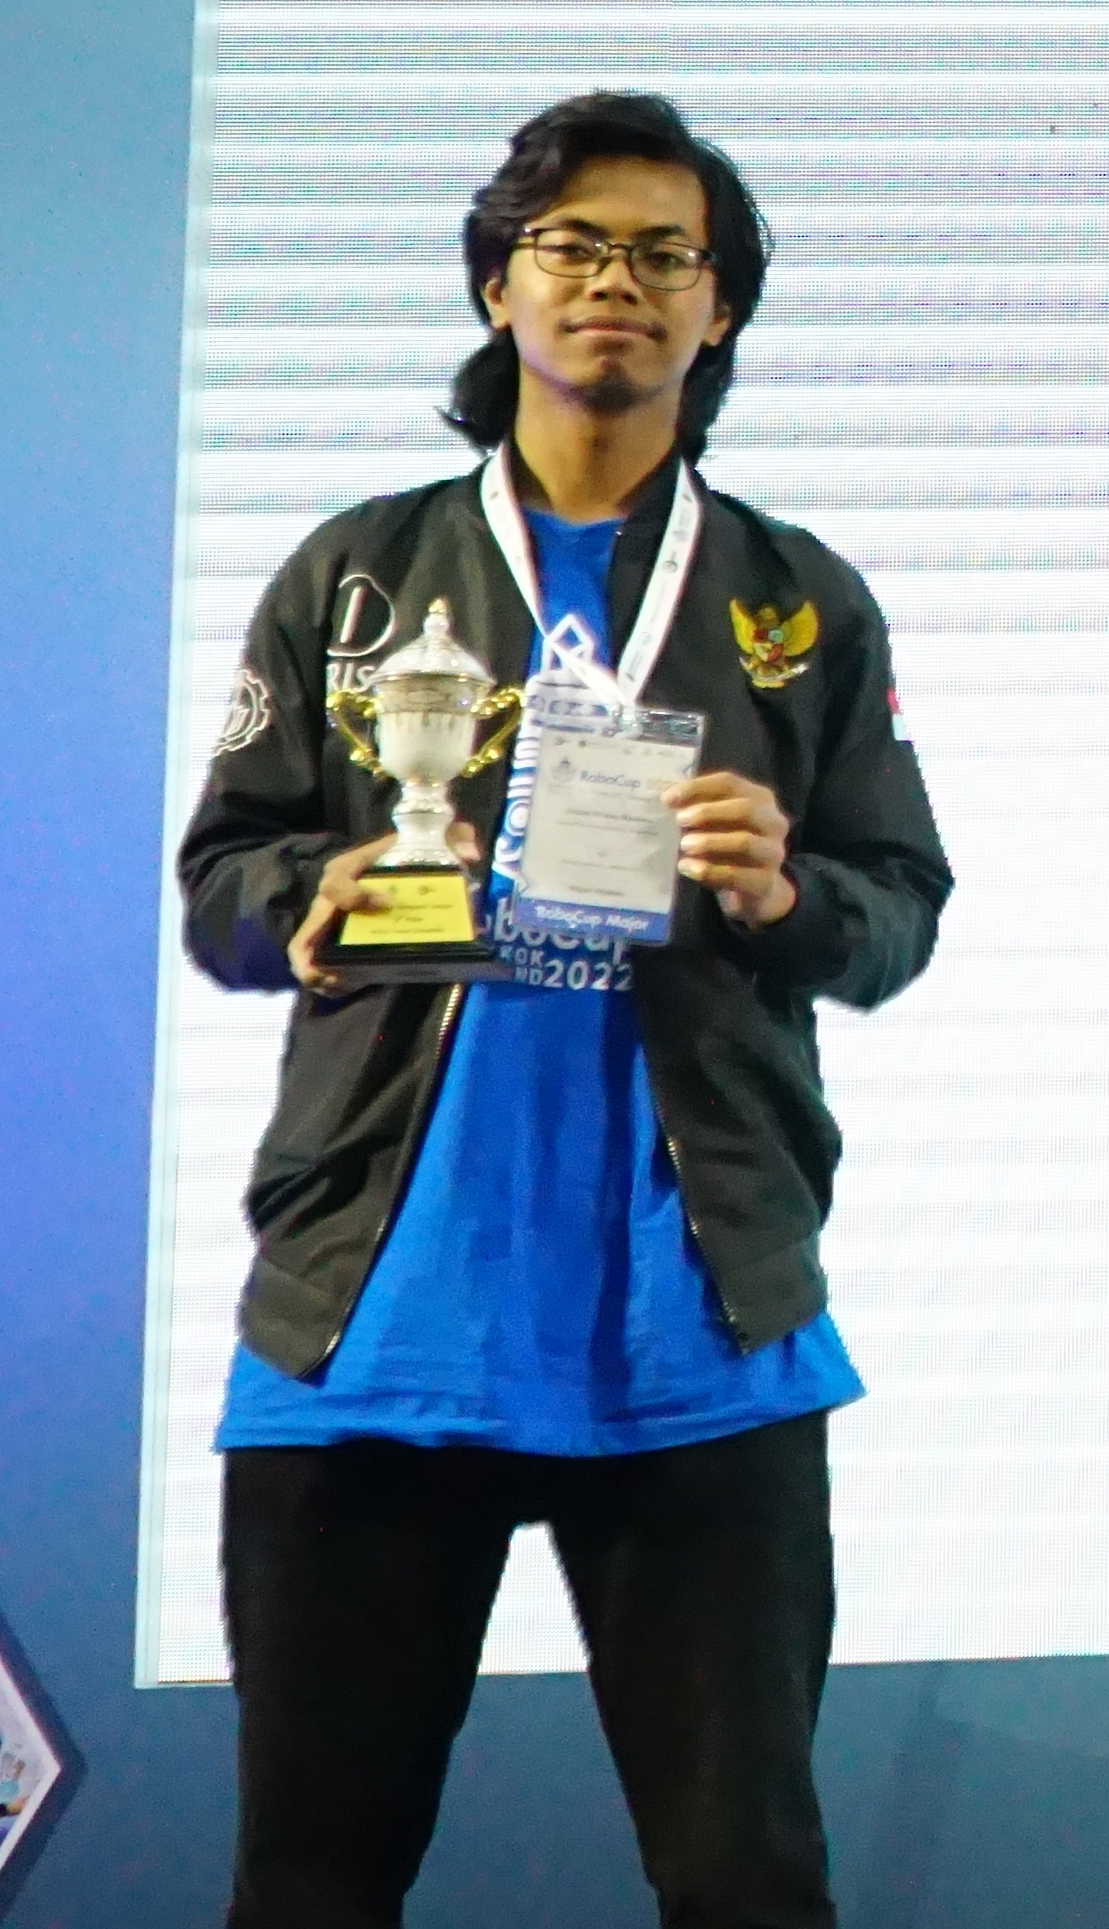
\includegraphics[height=0.2\textheight]{../ubah/Foto.jpg}
\end{center}
%*********************************

\section*{Personal Information}
\begin{tabular}{p{3cm}cp{9cm}}
    Name             & :& Azzam Widan Maulana \\
    Place of Birth   & :& Jember \\
    Date of Birth    & :& June 4, 2002 \\
    Address          & :& Arif Rahman Hakim Street No. 14A, Keputih, Sukolilo, Surabaya \\
\end{tabular}

\section*{Educational Background}
\begin{tabular}{p{3cm}cp{9cm}}
    2024–Present   & :& Master's Program (M.Sc.), Department of Electrical Engineering, Faculty of Intelligent Electrical and Informatics Technology, Institut Teknologi Sepuluh Nopember (ITS) \\
    &&\\
    2020–2024  & :& Bachelor Program (B.Eng.), Department of Computer Engineering, Faculty of Intelligent Electrical and Informatics Technology, Institut Teknologi Sepuluh Nopember (ITS) \\
    &&\\
    2017–2020  & :& SMAN 1 Jember \\
    &&\\
    2014–2017  & :& SMPN 3 Jember \\
    &&\\
    2008–2014  & :& SDN Kaliwates 2 Jember \\
    &&\\
    2006–2008  & :& TK Miftahul Ulum Kaliwates Jember \\
\end{tabular}

\section*{List of Publications}
\begin{enumerate}
    \item Muhtadin, A. W. Maulana, R. Dikairono and A. Zaini, "Omnivision Calibration on Mobile Robot Using Machine Learning," \textit{2024 International Conference on Computer Engineering, Network, and Intelligent Multimedia (CENIM)}, Surabaya, Indonesia, 2024, pp. 1–8, doi: 10.1109/CENIM64038.2024.10882712.
\end{enumerate}

\section*{Research History}
\begin{enumerate}
    \item Multicast Communication System on IRIS Robot 2022
    \item Natural Ball Handling System on IRIS Robot 2022
    \item Omnivision Camera Calibration on Mobile Robot Using Machine Learning 2023
    \item Robot Positioning System Using Gaussian Model on IRIS Robot 2023
    \item Empty Goal Detection System Using Omnivision Camera on IRIS Robot 2023
    \item Content Management System and User Interface for RAISA ITS Robot 2024
    \item Custom Operating System for Autonomous Vehicle and IRIS Robot 2024
    \item Empty Goal Detection System Using Stereo Depth Camera on IRIS Robot 2024
    \item Ball Detection System Using Spatial Image Classification on IRIS Robot 2024
    \item Hardware Communication System Using Layer 2 Communication for Autonomous Vehicle and IRIS Robot 2024
    \item Hardware Communication System Using CAN-bus for Autonomous Vehicle and IRIS Robot 2024
    \item End to End Machine Learning System for Autonomous Vehicle 2025
    \item Fleet Management System for AMR (Autonomous Mobile Robot) 2025
\end{enumerate}

\section*{Other Background}
Before venturing into the world of robotics and programming, the author was involved in music. As a musician, he mastered various musical instruments such as guitar, bass, and keyboard. In addition to playing instruments, he was also active in the field of mixing and mastering. His hobby of signal processing sparked an interest in learning how computers process signals. This passion led him to pursue a degree in Computer Engineering at ITS. Moreover, he delved into robotics to understand how computers and hardware operate, enabling him to perform advanced digital signal processing techniques.
